\uuid{QR6Q}
\exo7id{77}
\titre{exo7 77}
\auteur{bodin}
\organisation{exo7}
\datecreate{1998-09-01}
\video{wHlb0IsMB7Q}
\isIndication{false}
\isCorrection{true}
\chapitre{Nombres complexes}
\sousChapitre{Géométrie}
\module{Algèbre}
\niveau{L1}
\difficulte{}

\contenu{
\texte{
Soit $(A_{0},A_{1},A_{2},A_{3},A_{4})$ un pentagone r\'egulier. On note $O$ son centre et on
choisit un rep\`ere orthonorm\'e $(O,\overrightarrow{u},\overrightarrow{v})$ avec
$\overrightarrow{u}=\overrightarrow{OA_{0}}$, qui nous permet d'identifier le plan avec
l'ensemble des nombres complexes $\Cc$.
%dessin
$$
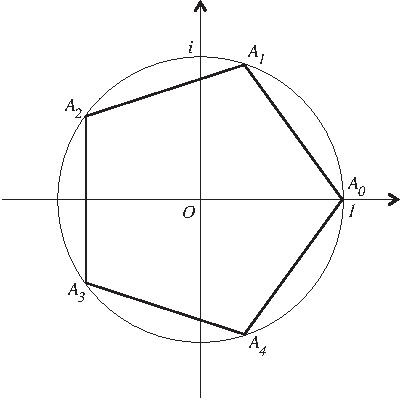
\includegraphics{../images/pdf/QR6Q-1.pdf}
$$
}
\begin{enumerate}
    \item \question{Donner les affixes $\omega_{0},\ldots,\omega_{4}$ des points $A_{0},\ldots,A_{4}$. Montrer
que  $\omega_{k}={\omega_{1}}^k$ pour $ k\in\{0,1,2,3,4\}$. Montrer que
$1+\omega_{1}+\omega_{1}^2+\omega_{1}^3+\omega_{1}^4=0$.}
\reponse{Comme $(A_{0},\ldots,A_{4})$ est un pentagone r\'egulier, on a
$OA_{0}=OA_{1}=OA_{2}=OA_{3}=OA_{4}=1$ et $
  (\overrightarrow{OA_{0}},\overrightarrow{OA_{1}})=\frac{2\pi}{5}[2\pi],
  (\overrightarrow{OA_{0}},\overrightarrow{OA_{2}})=\frac{4\pi}{5}[2\pi],
  (\overrightarrow{OA_{0}},\overrightarrow{OA_{3}})=-\frac{4\pi}{5}[2\pi],
  (\overrightarrow{OA_{0}},\overrightarrow{OA_{4}})=-\frac{2\pi}{5}[2\pi],
 $.
On en d\'eduit:
 $
  \omega_{0}=1,
  \omega_{1}=e^{\frac{2i\pi}{5}},
  \omega_{2}=e^{\frac{4i\pi}{5}},
  \omega_{3}=e^{-\frac{4i\pi}{5}}=e^{\frac{6i\pi}{5}},
  \omega_{4}=e^{-\frac{2i\pi}{5}}=e^{\frac{8i\pi}{5}},
 $.
On a bien $\omega_{i}=\omega_{1}^i$. Enfin, comme
$\omega_{1}\neq0$, $1+\omega_{1}+\ldots+\omega_{1}^4=
\frac{1-\omega_{1}^5}{1-\omega_{1}}=\frac{1-1}{1-\omega_{1}}=0$.}
    \item \question{En d\'eduire que $\cos(\frac{2\pi}{5})$ est l'une des solutions de l'\'equation $4z^2+2z-1=0$.
En d\'eduire la valeur de $\cos(\frac{2\pi}{5})$.}
\reponse{$\mathop{\mathrm{Re}}\nolimits(1+\omega_{1}+\ldots+\omega_{1}^4)=
1+2\cos(\frac{2\pi}{5})+2\cos(\frac{4\pi}{5})$. Comme
$\cos(\frac{4\pi}{5})=2\cos^2(\frac{2\pi}{5})-1$ on en d\'eduit:
$4\cos^2(\frac{2\pi}{5})+2\cos(\frac{2\pi}{5})-1=0$.
$\cos(\frac{2\pi}{5})$ est donc bien une solution de l'\'equation
$4z^2+2z-1=0$. Etudions cette \'equation: $\Delta=20=2^2.5$. Les
solutions sont donc $\frac{-1-\sqrt{5}}{4}$ et
$\frac{-1+\sqrt{5}}{4}$. Comme $\cos(\frac{2\pi}{5})>0$, on en
d\'eduit que $\cos(\frac{2\pi}{5})=\frac{\sqrt{5}-1}{4}$.}
    \item \question{On consid\`ere le point $B$ d'affixe $-1$. Calculer la longueur $BA_{2}$ en fonction de
$\sin\frac{\pi}{10}$ puis de $\sqrt{5}$ (on remarquera que
$\sin\frac{\pi}{10}=\cos\frac{2\pi}{5}$).}
\reponse{$
  BA_{2}^2=|\omega_{2}+1|^2
          =|\cos(\frac{4\pi}{5})+i\sin(\frac{4\pi}{5})+1|^2
          =1+2\cos(\frac{4\pi}{5})+\cos^2(\frac{4\pi}{5})+\sin^2(\frac{4\pi}{5})
          =4\cos^2(\frac{2\pi}{5})
  $. Donc $BA_{2}=\frac{\sqrt{5}-1}{2}$.}
    \item \question{On consid\`ere le point $I$ d'affixe $\frac{i}{2}$, le cercle $\mathcal{C}$ de centre $I$ de
rayon $\frac{1}{2}$ et enfin le point $J$ d'intersection de $\mathcal{C}$ avec le segment
$[BI]$. Calculer la longueur $BI$ puis la longueur $BJ$.}
\reponse{$BI=|i/2+1|=\frac{\sqrt{5}}{2}$. $BJ=BI-1/2=\frac{\sqrt{5}-1}{2}$.}
    \item \question{\textbf{Application:} Dessiner un pentagone r\'egulier \`a la r\`egle et au compas. Expliquer.}
\reponse{Pour tracer un pentagone r\'egulier, on commence par tracer un
cercle $C_{1}$ et deux diam\`etres orthogonaux, qui jouent le r\^ole
du cercle passant par les sommets et des axes de coordonn\'ees. On
trace ensuite le milieu d'un des rayons: on obtient le point I de
la question 4. On trace le  cercle de centre $I$ passant par le
centre de $C_{1}$: c'est le cercle $\mathcal{C}$. On trace le
segment $BI$ pour obtenir son point $J$ d'intersection avec
$\mathcal{C}$. On trace enfin le cercle de centre $B$ passant par
$J$: il coupe $C_{1}$ en $A_{2}$ et $A_{3}$, deux sommets du
pentagone. Il suffit pour obtenir tous les sommets de reporter la
distance $A_{2}A_{3}$ sur $C_{1}$, une fois depuis $A_{2}$, une
fois depuis $A_{3}$. (en fait le cercle de centre $B$ et passant
par $J'$, le point de $\mathcal{C}$ diam\'etralement oppos\'e \`a
$J$, coupe $C_{1}$ en $A_{1}$ et $A_{4}$, mais nous ne l'avons pas
justifi\'e par le calcul : c'est un exercice !)}
\end{enumerate}
}
